% Copyright 2021 Fausto Spoto
%
% Licensed under the Apache License, Version 2.0 (the "License");
% you may not use this file except in compliance with the License.
% You may obtain a copy of the License at
%
%    http://www.apache.org/licenses/LICENSE-2.0
%
% Unless required by applicable law or agreed to in writing, software
% distributed under the License is distributed on an "AS IS" BASIS,
% WITHOUT WARRANTIES OR CONDITIONS OF ANY KIND, either express or implied.
% See the License for the specific language governing permissions and
% limitations under the License.

\documentclass[11pt]{beamer}  %% versione proiettore
%%\documentclass[11pt,handout]{beamer} %% versione stampa
\usepackage{lucidiJb-2ed}
\usepackage{mathtools}
\usepackage{relsize}
\usepackage[normalem]{ulem}

\mode<article>
{
  \usepackage{fullpage}
  \usepackage{hyperref}
}

\mode<presentation>
{
  \setbeamertemplate{background canvas}[vertical shading][bottom=red!10,top=blue!10]
  \usetheme{Course}
  \usefonttheme[onlysmall]{structurebold}
}

\subtitle{Blockchain Course}
\title{Tendermint}
\institute{Universit\`a di Verona, Italy}
\date{October 2024}

\setbeamercovered{invisible}

\def\codesize{\smaller}
\def\<#1>{\codeid{#1}}
\newcommand{\codeid}[1]{\ifmmode{\mbox{\codesize\ttfamily{#1}}}\else{\codesize\ttfamily #1}\fi}

\begin{document}

\begin{frame}
  \titlepage
\end{frame}

\begin{frame}
  \frametitle{Proof of\ldots}

  \begin{center}
    Who decides the next block?
  \end{center}

  \bigskip

  \begin{greenbox}{Proof-of-work [PoW] is expensive and leads to forks}
    \begin{itemize}
    \item proof-of-stake [PoS] (who stakes the most)
    \item proof-of-space (who consumes more memory)
    \item proof-of-authority (who has more authority)
    \item \ldots
    \end{itemize}
  \end{greenbox}

  \bigskip

  \begin{greenbox}{PoS is a variant of Practical Byzantine Fault Tolerance (BFT)}
    Miguel Castro and Barbara Liskov.
    \emph{Practical Byzantine Fault Tolerance and Proactive Recovery}.
    ACM Trans.\ Comput.\ Syst., 20(4):398–461, November 2002
  \end{greenbox}

\end{frame}

\begin{frame}\frametitle{Tendermint (\url{https://tendermint.com/})}

  \begin{greenbox}{Jae Kwon. \emph{Tendermint: Consensus without Mining}, 2014.\\
    \url{https://tendermint.com/static/docs/tendermint.pdf}}
    \begin{itemize}
    \item a dynamic set $V$ of validators decides the next block
    \item $V$ might be different for each block
      \begin{itemize}
      \item but deterministically computed from the previous history
      \end{itemize}
    \item at each height $H$, each validator $v\in V$:
      \begin{enumerate}
      \item identifies (deterministically) a validator $m\in V$ that
        is expected to aggregate some transactions and \alert{propose} a next block $b$
      \item if it considers $b$ valid, it \alert{pre-votes} $b$
      \item counts how many validators pre-vote $b$
      \item if it counts at least $\frac{2}{3}$ pre-votes, it \alert{pre-commits} $b$
      \item counts how many validators pre-commit $b$
      \item if it counts at least $\frac{2}{3}$ pre-commits, it \alert{commits} $b$ and increases $H$
      \item goes back to step~1
      \end{enumerate}
    \end{itemize}
  \end{greenbox}

  \smallskip

  \begin{center}
    Tendermint is BFT. If step~1 is based on stakes, then it is PoS
  \end{center}

\end{frame}

\begin{frame}\frametitle{Tendermint's polka}

  \begin{center}
    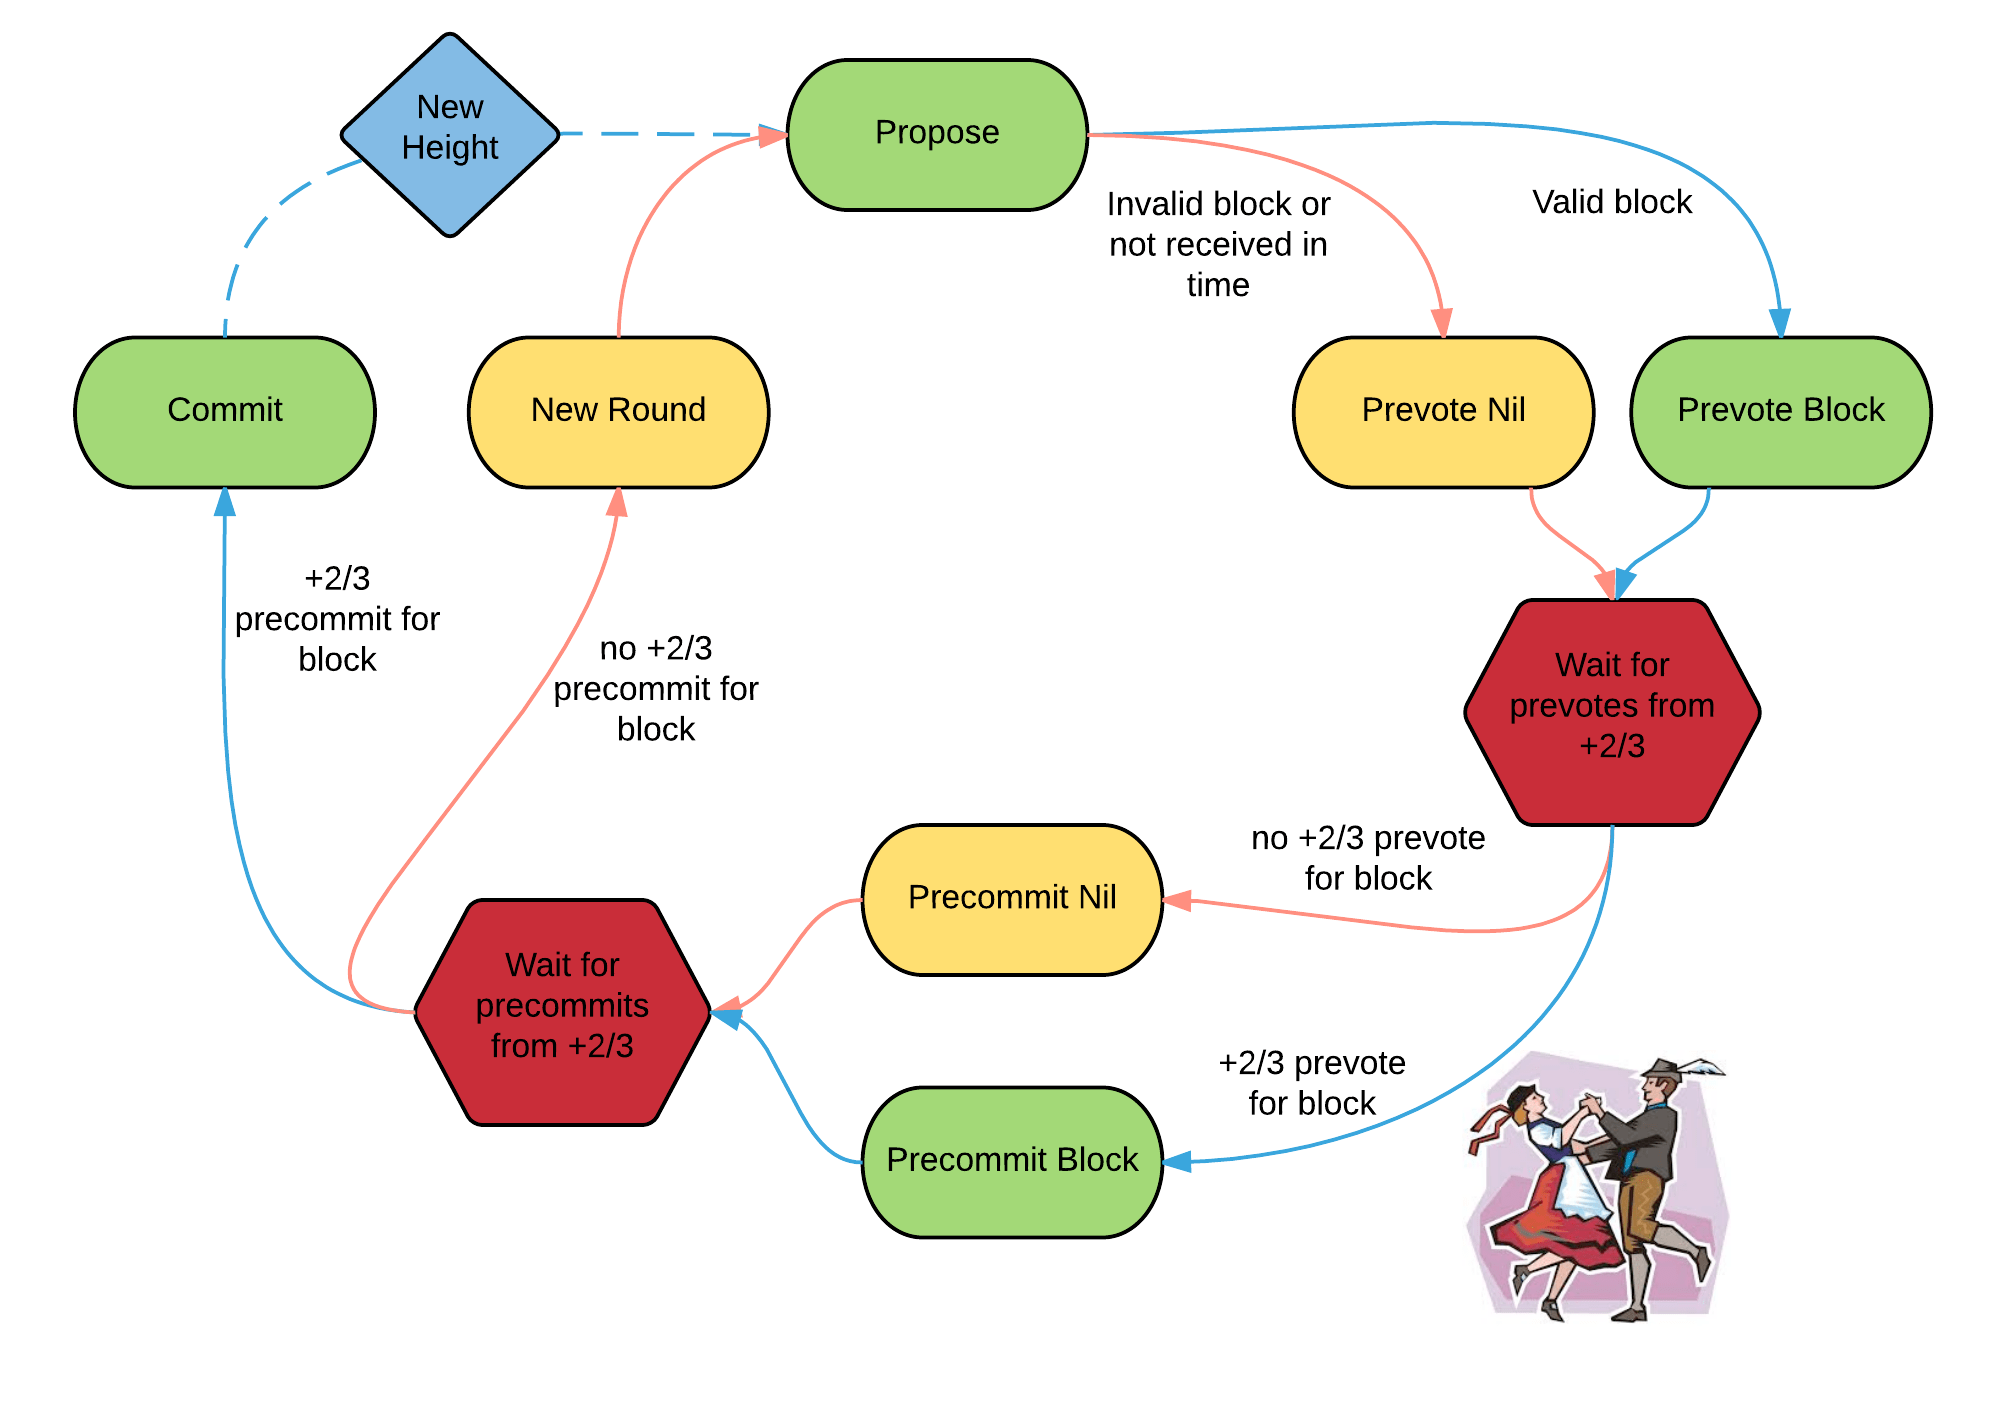
\includegraphics[scale=.15,clip=false]{pictures/polka.png}
  \end{center}

\end{frame}

\begin{frame}\frametitle{The mempool}

  \begin{center}
    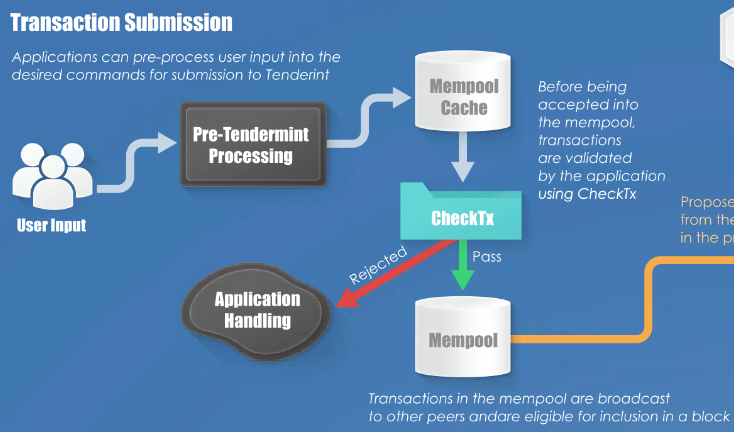
\includegraphics[scale=.4,clip=false]{pictures/tendermint-mempool.png}
  \end{center}

  \begin{center}
    \<checkTx(tx)> checks if the transaction \<tx> is valid
  \end{center}

\end{frame}

\begin{frame}\frametitle{Pre-vote}

  \begin{center}
    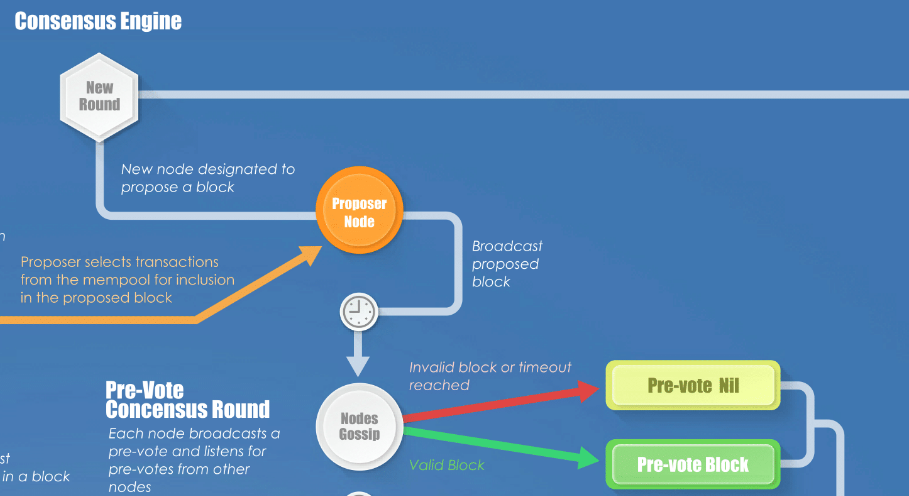
\includegraphics[scale=.38,clip=false]{pictures/tendermint-prevote.png}
  \end{center}

  \begin{center}
    \<checkTx(tx)> again + \<deliverTx(tx)> to check if the block is valid
  \end{center}

\end{frame}

\begin{frame}\frametitle{Pre-commit}

  \begin{center}
    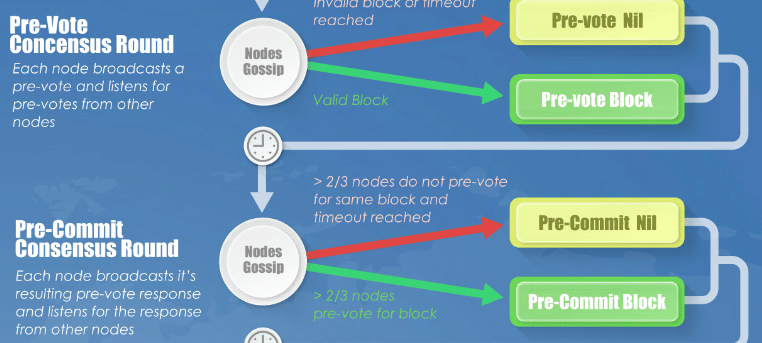
\includegraphics[scale=.43,clip=false]{pictures/tendermint-precommit.png}
  \end{center}

\end{frame}

\begin{frame}\frametitle{Commit}

  \begin{center}
    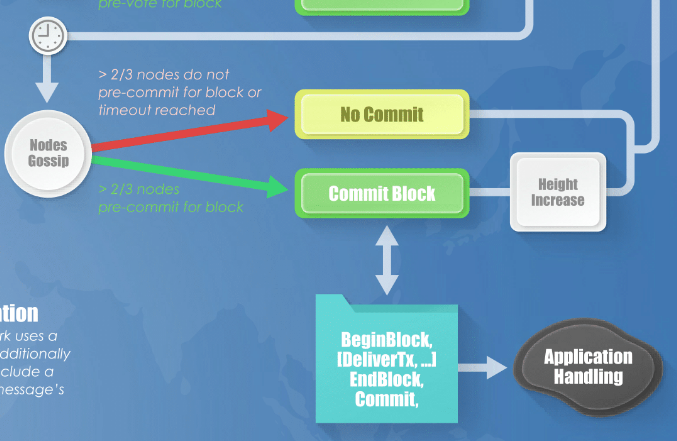
\includegraphics[scale=.38,clip=false]{pictures/tendermint-commit.png}
  \end{center}

  \begin{center}
    \<commit()> stores the state at the end of the block
  \end{center}

\end{frame}

\begin{frame}\frametitle{Next round, or next height}

  \begin{center}
    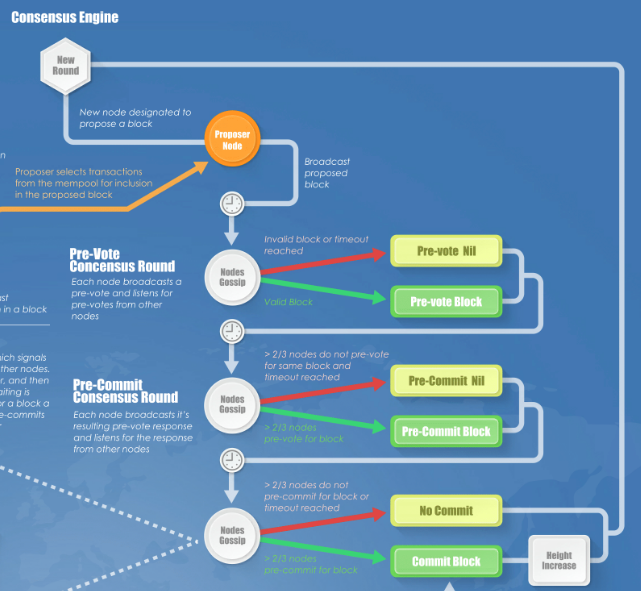
\includegraphics[scale=.36,clip=false]{pictures/tendermint-consensus.png}
  \end{center}

\end{frame}

\begin{frame}\frametitle{Inside a Tendermint block}

  \begin{center}
    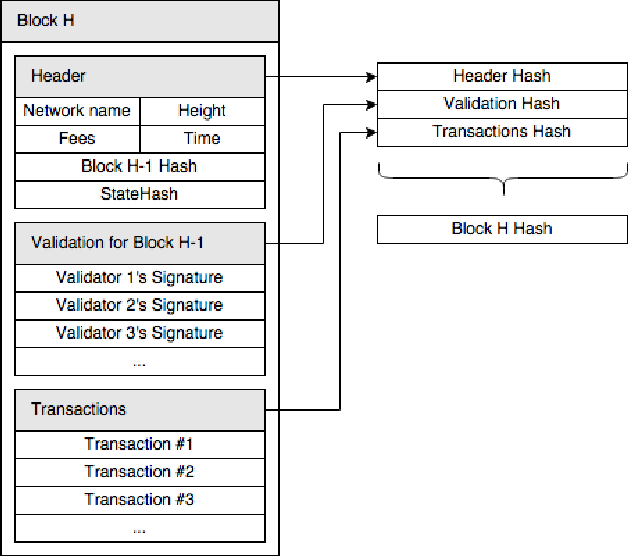
\includegraphics[scale=.38,clip=false]{pictures/tendermint-block.png}
  \end{center}

\end{frame}

\begin{frame}\frametitle{A layered implementation in Golang}

  \begin{center}
    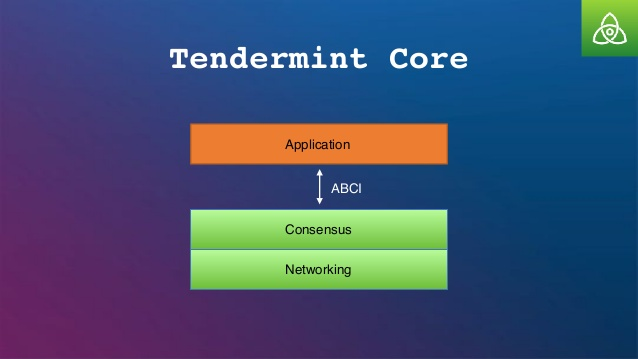
\includegraphics[scale=.38,clip=false]{pictures/tendermint-core.jpg}
  \end{center}

  \begin{center}
    ABCI: Application BlockChain Interface
  \end{center}

\end{frame}

\begin{frame}\frametitle{The application layer}

  \begin{center}
    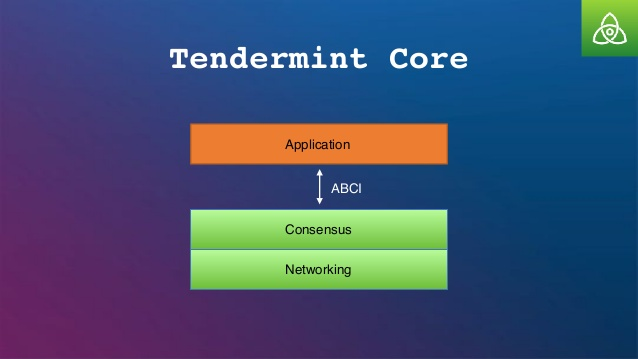
\includegraphics[scale=.15,clip=false]{pictures/tendermint-core.jpg}
  \end{center}
  
  \begin{greenbox}{The application layer is not part of Tendermint Core}
    Programmers can write their own application layer
    \begin{itemize}
    \item connected to Tendermint Core via ABCI using sockets
    \item possibly on a different machine than Tendermint Core
    \item in any programming language
    \end{itemize}
  \end{greenbox}

  \bigskip

  \begin{redbox}{}
    \begin{center}
      The application layer must be deterministic!
    \end{center}
  \end{redbox}

\end{frame}

\begin{frame}\frametitle{The ABCI}

  \begin{center}
    \url{https://docs.tendermint.com/master/spec/abci/abci.html}
  \end{center}

  \begin{itemize}
  \item[] \alert{\<checkTx>}: called before entering the mempool and to verify blocks
    \begin{itemize}
    \item[$\Rightarrow$] only transactions that satisfy \<checkTx> are added in blocks
    \item[{
\includegraphics[scale=0.0135]{pictures/uncheck.png}}] must not modify the state of the application
    \end{itemize}
    \hrule
  \item[] \alert{\<beginBlock>}: called at the beginning of a block; receives information
    about the validator set of the previous block and which of them signed the previous block
  \item[] \alert{\<deliverTx>}: called for each transaction added to a block: it executes
    the transaction by modifying the state of the application
  \item[] \alert{\<endBlock>}: called at the end of a block; provides information
    about the validator set for the next block
  \item[] \alert{\<commit>}: called when a block is being committed; it stores the state of the application in the database and provides its hash
    \hrule
  \item[] \alert{\<query>}: called when the user wants to read data from the blockchain
  \end{itemize}
\end{frame}

\begin{frame}\frametitle{The ABCI}

  \begin{center}
    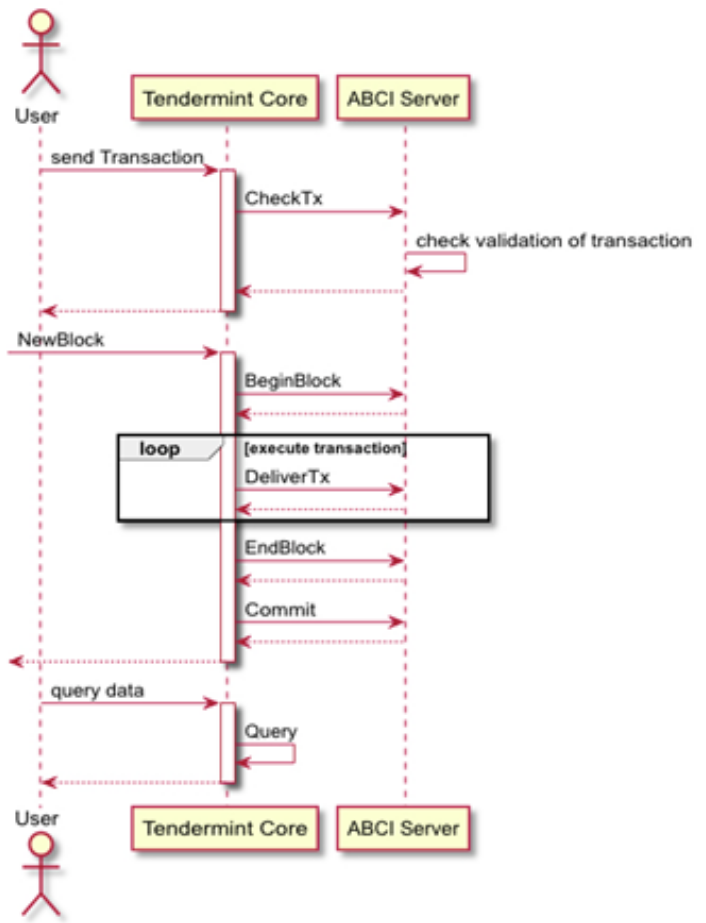
\includegraphics[scale=.2,clip=false]{pictures/abci.png}
  \end{center}

  \begin{redbox}{}
    State updates between \<beginBlock> and \<commit> must be seen as a single atomic update
    of the application state
  \end{redbox}

\end{frame}

\begin{frame}\frametitle{The database of blocks and the application state}

  \begin{center}
    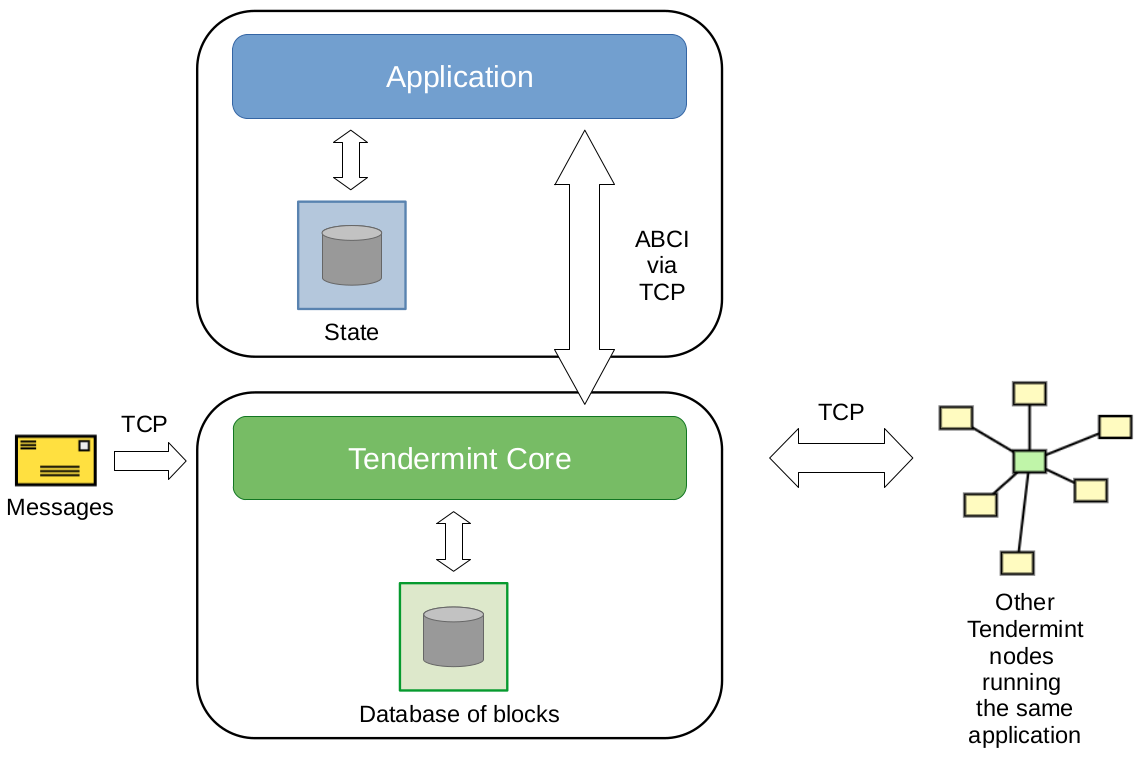
\includegraphics[width=\textwidth,clip=false]{pictures/tendermint-databases.png}
  \end{center}

\end{frame}

\begin{frame}\frametitle{The application state}

  \begin{greenbox}{It must have a function to compute its hash}
    Only that hash is reported in blockchain, for consensus
  \end{greenbox}

  \bigskip

  \begin{greenbox}{It must allow transactional, atomic updates}
    Between \<beginBlock> and \<commit>
  \end{greenbox}

  \bigskip

  \begin{greenbox}{The API of the state}
    Tendermint enjoys finality: there are no forks
    \begin{itemize}
      \item[$\Rightarrow$] one never needs to come
        back in time to the state of a previous block
    \end{itemize}

    \begin{enumerate}
    \item get data
    \item put data
    \item \<h=get\_hash()>
    \item \sout{\<checkout(h)>} $\Rightarrow$ big opportunity for garbage collection!
    \end{enumerate}
  \end{greenbox}

\end{frame}

\begin{frame}\frametitle{Cosmos: a Tendermint application in Golang}

  \begin{center}
    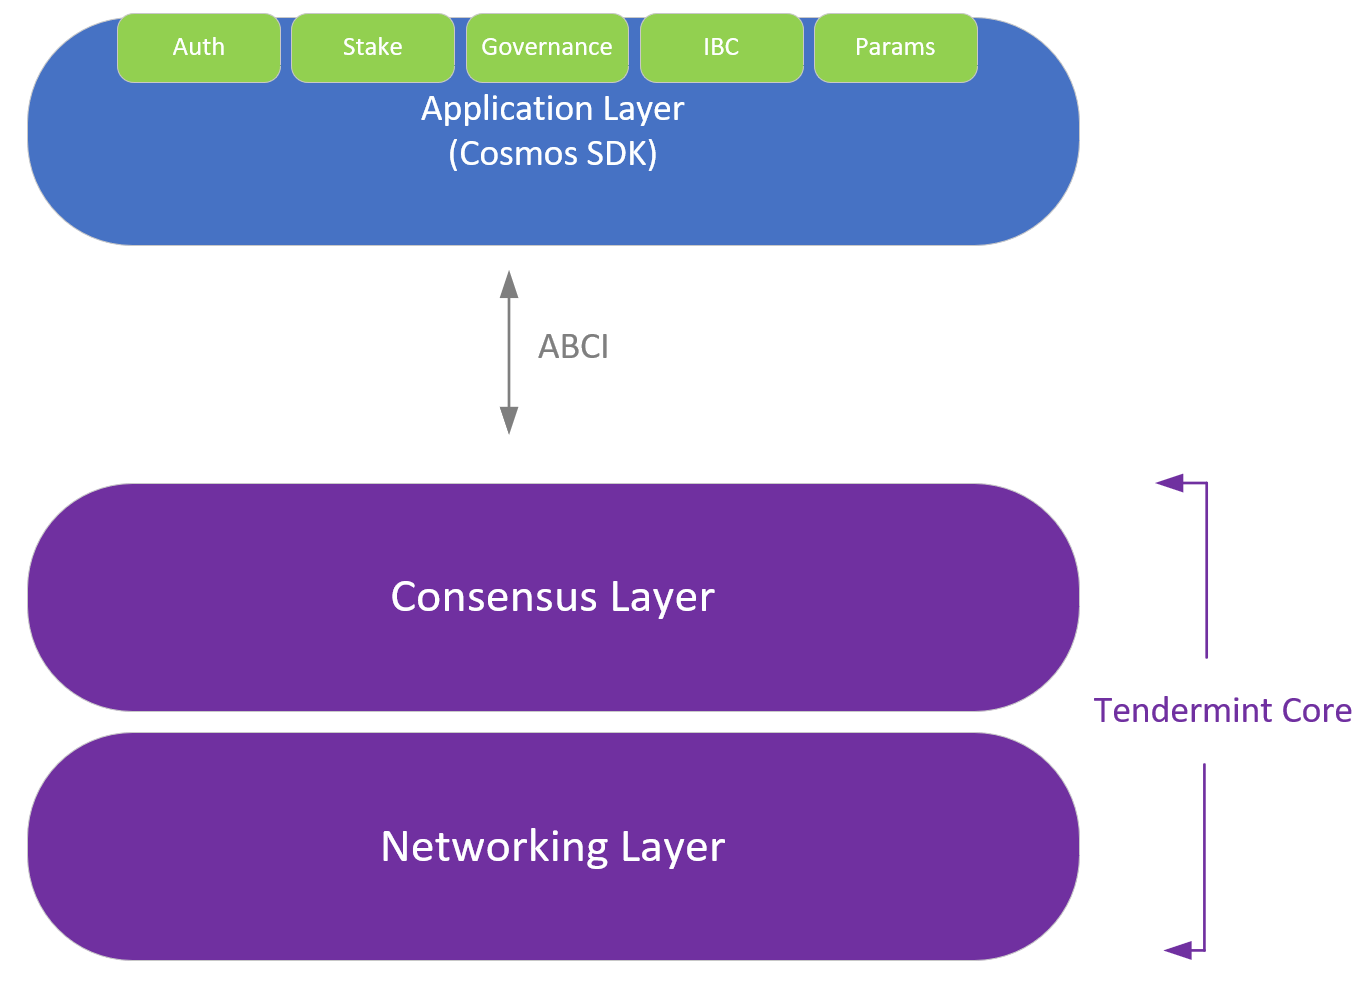
\includegraphics[scale=0.2,clip=false]{pictures/cosmos.png}
  \end{center}

\end{frame}

\begin{frame}\frametitle{The application state of Cosmos}

  \begin{greenbox}{Cosmos keeps data inside \alert{keepers}}
    They are maps $\mathit{key}\to\mathit{value}$. Programmers must store
    persistent data inside a keeper: all other data is lost if the node
    is turned off and on again
  \end{greenbox}

  \bigskip

  \begin{greenbox}{Golang}
    Cosmos can be expanded with arbitrary Golang code, but:
    \begin{itemize}
    \item it must be deterministic
    \item it must store persistent data in a keeper
    \item it must count gas consumption explicitly
    \end{itemize}
  \end{greenbox}

  \bigskip

  \begin{greenbox}{Smart contracts?}
    There are no smart contracts in Cosmos, really. The system as a whole
    is a big (fixed) smart contract
    \begin{itemize}
    \item[$\Rightarrow$] maintenance issue
    \end{itemize}
  \end{greenbox}

\end{frame}

\end{document}
